\documentclass[12pt, titlepage]{article}

\usepackage{fullpage}
\usepackage[round]{natbib}
\usepackage{multirow}
\usepackage{booktabs}
\usepackage{tabularx}
\usepackage{graphicx}
\usepackage{float}
\usepackage{hyperref}
\hypersetup{
    colorlinks,
    citecolor=blue,
    filecolor=black,
    linkcolor=red,
    urlcolor=blue
}

\input{../../Comments.text}
\input{../../Common.text}

\newcounter{acnum}
\newcommand{\actheacnum}{AC\theacnum}
\newcommand{\acref}[1]{AC\ref{#1}}

\newcounter{ucnum}
\newcommand{\uctheucnum}{UC\theucnum}
\newcommand{\uref}[1]{UC\ref{#1}}

\newcounter{mnum}
\newcommand{\mthemnum}{M\themnum}
\newcommand{\mref}[1]{M\ref{#1}}

\begin{document}

\title{Module Guide for \progname{}} 
\author{\authname}
\date{\today}

\maketitle

\pagenumbering{roman}

\section{Revision History}

\begin{tabularx}{\textwidth}{p{3cm}p{2cm}X}
\toprule {\bf Date} & {\bf Version} & {\bf Notes}\\
\midrule
Nov 5, 2026 & 1.0 & Davis Lenover: Revision $-1$. Sections 1 to 3, 5
Module Hierarchy, 7 Module Decomposition for the kernel, market and trading,
and 9 Use Hierarchy Between Modules.\\
Nov 9, 2026 & 1.1 & Davis Lenover: Email Service (M25) in 5 Module
Hierarchy. 7 Module Decomposition: Users, Wallet and Email Service, a rationale
for each module, and module health in Control and Plugins. Review fixes to Database, Market,
Trading (queued trades and the simulation notice at Revision~0) and JSON
Format, and to 9 Use Hierarchy Between Modules.\\
\bottomrule
\end{tabularx}

\newpage

\section{Reference Material}

This section records information for easy reference. 

\subsection{Abbreviations and Acronyms}

\renewcommand{\arraystretch}{1.2}
\begin{tabular}{l l} 
  \toprule		
  \textbf{symbol} & \textbf{description}\\
  \midrule 
  AC & Anticipated Change\\
  API & Application Programming Interface\\
  DAG & Directed Acyclic Graph\\
  \progname & A phone app where physical activity earns virtual currency\\
   & that the user invests in a simulated stock market\\
  FR & Functional Requirement (SRS)\\
  HA & Hazard Analysis\\
  JSON & JavaScript Object Notation\\
  LC & Likely Change (SRS)\\
  M & Module\\
  MG & Module Guide\\
  MIS & Module Interface Specification\\
  NFR & Nonfunctional Requirement (SRS)\\
  OS & Operating System\\
  PoC & Proof of Concept\\
  REST & Representational State Transfer\\
  SC & System Constraint (SRS)\\
  SEC & Security Requirement (SRS and HA)\\
  SRS & Software Requirements Specification\\
  UC & Unlikely Change\\
  \bottomrule
\end{tabular}\\

\newpage

\tableofcontents

\listoftables

\listoffigures

\newpage

\pagenumbering{arabic}

\section{Introduction}

\progname{} joins two things that are usually kept apart: fitness and
investing. Activity recorded on the phone earns virtual currency, the user
spends it on simulated stocks priced from a real market, and the results feed
goals, learning content and a social feed. That brings three design
challenges:

\begin{itemize}
\item The features depend on each other. A user buying a stock needs the
  latest price from the market and their balance from the wallet, and must
  change both the balance and the shares together. Activity rewards land in
  the same wallet. The social feed shares activity and milestones, but must
  never show a balance or health data.
\item Some parts rely on outside services that may change: the market data
  provider, which allows users to buy shares in the first place, and the health
  platforms on iOS and Android.
\item Given this is a group project, the system will be developed in parallel,
  in stages, from the proof of concept to Revision 1.
\end{itemize}

When we first designed the backend, we routed commands to different services
and let those services talk to each other directly, each with its own
libraries. Taking a step back, this greatly increased coupling: a logic change
in any one of these modules could easily ripple through the others. We needed
a way to separate the modules, so that each one keeps its data and its
decisions to itself, and the others reach it only through a small interface.
This helps to support changes and additions to the modules.

Decomposing a system into modules is a commonly accepted approach to developing
software. We decompose \progname{} by information hiding: each module hides a
``secret'', a design decision that is likely to change, such as the market data
provider or a health platform. Separate modules also naturally become work
assignments that people can develop in tandem. With a defined interface in
between, it becomes much easier to work in parallel.

\progname{} is two programs: a server, written in Python with FastAPI and
backed by PostgreSQL, and a phone app, written in React Native. The phone app
talks to the server over HTTPS with JSON. This MG covers the modules of both
programs.

Our design follows three rules:
\begin{itemize}
\item System details that are likely to change independently should be the
  secrets of separate modules.
\item Each data structure is implemented in only one module.
\item Any other program that requires information stored in a module's data
  structures must obtain it by calling access programs belonging to that module.
\end{itemize}

After completing the first stage of the design, the Software Requirements
Specification (SRS), the Module Guide (MG) is developed. The MG
specifies the modular structure of the system and is intended to allow both
designers and maintainers to easily identify the parts of the software.  The
potential readers of this document are as follows:

\begin{itemize}
\item New project members: This document can be a guide for a new project member
  to easily understand the overall structure and quickly find the
  relevant modules they are searching for.
\item Maintainers: The hierarchical structure of the module guide improves the
  maintainers' understanding when they need to make changes to the system. It is
  important for a maintainer to update the relevant sections of the document
  after changes have been made.
\item Designers: Once the module guide has been written, it can be used to
  check for consistency, feasibility, and flexibility. Designers can verify the
  system in various ways, such as consistency among modules, feasibility of the
  decomposition, and flexibility of the design.
\end{itemize}

The rest of the document is organized as follows. Section
\ref{SecChange} lists the anticipated and unlikely changes of the software
requirements. Section \ref{SecMH} summarizes the module decomposition that
was constructed according to the likely changes. Section \ref{SecConnection}
specifies the connections between the software requirements and the
modules. Section \ref{SecMD} gives a detailed description of the
modules. Section \ref{SecTM} includes two traceability matrices. One checks
the completeness of the design against the requirements provided in the SRS. The
other shows the relation between anticipated changes and the modules. Section
\ref{SecUse} describes the use relation between modules. The remaining sections
cover the user interfaces, the communication protocols, the database design and
the timeline.

\section{Anticipated and Unlikely Changes} \label{SecChange}

This section lists possible changes to the system. According to the likeliness
of the change, the possible changes are classified into two
categories. Anticipated changes are listed in Section \ref{SecAchange}, and
unlikely changes are listed in Section \ref{SecUchange}.

\subsection{Anticipated Changes} \label{SecAchange}

Anticipated changes are the source of the information that is to be hidden
inside the modules. Ideally, changing one of the anticipated changes will only
require changing the one module that hides the associated decision. The approach
adapted here is called design for
change.

\begin{description}
\item[\refstepcounter{acnum} \actheacnum \label{acHardware}:] The specific
  hardware on which the software is running.
\item[\refstepcounter{acnum} \actheacnum \label{acInput}:] The format of the
  initial input data.
\item ...
\end{description}

\wss{Anticipated changes relate to changes that would be made in requirements,
design or implementation choices.  They are not related to changes that are made
at run-time, like the values of parameters.}

\subsection{Unlikely Changes} \label{SecUchange}

The module design should be as general as possible. However, a general system is
more complex. Sometimes this complexity is not necessary. Fixing some design
decisions at the system architecture stage can simplify the software design. If
these decision should later need to be changed, then many parts of the design
will potentially need to be modified. Hence, it is not intended that these
decisions will be changed.

\begin{description}
\item[\refstepcounter{ucnum} \uctheucnum \label{ucIO}:] Input/Output devices
  (Input: File and/or Keyboard, Output: File, Memory, and/or Screen).
\item ...
\end{description}

\section{Module Hierarchy} \label{SecMH}

This section provides an overview of the module design. Modules are summarized
in a hierarchy decomposed by secrets in Table \ref{TblMH}. The modules listed
below, which are leaves in the hierarchy tree, are the modules that will
actually be implemented.

The hierarchy covers both programs in \progname{}, the server and the phone
app. Modules that are only in the app are marked (app). Hardware-hiding modules
hide the interfaces of software and devices the team does not write. These are
the database server, the server's clock, the market data provider, the email
service, and the phone's health platform and operating system. Behaviour-hiding modules hide the
behaviour the SRS describes. Software decision modules hide choices the team
made that the SRS does not mention.

\begin{description}
% Hardware-Hiding
\item [\refstepcounter{mnum} \mthemnum \label{mDB}:] Database
\item [\refstepcounter{mnum} \mthemnum \label{mClock}:] Clock
\item [\refstepcounter{mnum} \mthemnum \label{mProviders}:] Market Providers
\item [\refstepcounter{mnum} \mthemnum \label{mHealth}:] Health Service (app)
\item [\refstepcounter{mnum} \mthemnum \label{mDevice}:] Device Service (app)
% Behaviour-Hiding, server
\item [\refstepcounter{mnum} \mthemnum \label{mControl}:] Control
\item [\refstepcounter{mnum} \mthemnum \label{mConstants}:] Constants (server and app)
\item [\refstepcounter{mnum} \mthemnum \label{mUsers}:] Users
\item [\refstepcounter{mnum} \mthemnum \label{mWallet}:] Wallet
\item [\refstepcounter{mnum} \mthemnum \label{mMarket}:] Market
\item [\refstepcounter{mnum} \mthemnum \label{mActivity}:] Activity
\item [\refstepcounter{mnum} \mthemnum \label{mTrading}:] Trading
\item [\refstepcounter{mnum} \mthemnum \label{mGoals}:] Goals\textsuperscript{\dag}
\item [\refstepcounter{mnum} \mthemnum \label{mLearning}:] Learning\textsuperscript{\dag}
\item [\refstepcounter{mnum} \mthemnum \label{mSocial}:] Social\textsuperscript{\dag}
\item [\refstepcounter{mnum} \mthemnum \label{mScenarios}:] Scenarios\textsuperscript{\dag}
\item [\refstepcounter{mnum} \mthemnum \label{mPrivacy}:] Privacy\textsuperscript{\dag}
% Behaviour-Hiding, app
\item [\refstepcounter{mnum} \mthemnum \label{mNavigation}:] Navigation (app)
\item [\refstepcounter{mnum} \mthemnum \label{mScreens}:] Screens (app)
\item [\refstepcounter{mnum} \mthemnum \label{mSync}:] Sync Service (app)
\item [\refstepcounter{mnum} \mthemnum \label{mReminders}:] Reminder Service (app)\textsuperscript{\dag}
% Software Decision
\item [\refstepcounter{mnum} \mthemnum \label{mPlugins}:] Plugins
\item [\refstepcounter{mnum} \mthemnum \label{mJSON}:] JSON Format
\item [\refstepcounter{mnum} \mthemnum \label{mAPI}:] API Service (app)
% Hardware-Hiding, added last so no other module is renumbered
\item [\refstepcounter{mnum} \mthemnum \label{mEmail}:] Email Service\textsuperscript{\dag}
\end{description}

\begin{table}[h!]
\centering
\begin{tabular}{p{0.3\textwidth} p{0.6\textwidth}}
\toprule
\textbf{Level 1} & \textbf{Level 2}\\
\midrule

\multirow{6}{0.3\textwidth}{Hardware-Hiding Module} & \mref{mDB} Database\\
& \mref{mClock} Clock\\
& \mref{mProviders} Market Providers\\
& \mref{mEmail} Email Service\textsuperscript{\dag}\\
& \mref{mHealth} Health Service (app)\\
& \mref{mDevice} Device Service (app)\\
\midrule

\multirow{16}{0.3\textwidth}{Behaviour-Hiding Module} & \mref{mControl} Control\\
& \mref{mConstants} Constants (server and app)\\
& \mref{mUsers} Users\\
& \mref{mWallet} Wallet\\
& \mref{mMarket} Market\\
& \mref{mActivity} Activity\\
& \mref{mTrading} Trading\\
& \mref{mGoals} Goals\textsuperscript{\dag}\\
& \mref{mLearning} Learning\textsuperscript{\dag}\\
& \mref{mSocial} Social\textsuperscript{\dag}\\
& \mref{mScenarios} Scenarios\textsuperscript{\dag}\\
& \mref{mPrivacy} Privacy\textsuperscript{\dag}\\
& \mref{mNavigation} Navigation (app)\\
& \mref{mScreens} Screens (app)\\
& \mref{mSync} Sync Service (app)\\
& \mref{mReminders} Reminder Service (app)\textsuperscript{\dag}\\
\midrule

\multirow{3}{0.3\textwidth}{Software Decision Module} & \mref{mPlugins} Plugins\\
& \mref{mJSON} JSON Format\\
& \mref{mAPI} API Service (app)\\
\bottomrule

\end{tabular}
\caption{Module Hierarchy}
\label{TblMH}
\end{table}

Modules marked with \textsuperscript{\dag} in Table~\ref{TblMH} are built after
the proof of concept and are specified in the MIS at Revision~0.

\section{Connection Between Requirements and Design} \label{SecConnection}

The design of the system is intended to satisfy the requirements developed in
the SRS. In this stage, the system is decomposed into modules. The connection
between requirements and modules is listed in Table~\ref{TblRT}.

\wss{The intention of this section is to document decisions that are made
  ``between'' the requirements and the design.  To satisfy some requirements,
  design decisions need to be made.  Rather than make these decisions implicit,
  they are explicitly recorded here.  For instance, if a program has security
  requirements, a specific design decision may be made to satisfy those
  requirements with a password.}

\section{Module Decomposition} \label{SecMD}

Modules are decomposed according to the principle of ``information
hiding''. The \emph{Secrets} field in a module
decomposition is a brief statement of the design decision hidden by the
module. The \emph{Services} field specifies \emph{what} the module will do
without documenting \emph{how} to do it. For each module, a suggestion for the
implementing software is given under the \emph{Implemented By} title. If the
entry is \emph{OS}, this means that the module is provided by the operating
system or by standard programming language libraries.  \emph{\progname{}} means the
module will be implemented by the \progname{} software.

Only the leaf modules in the hierarchy have to be implemented. If a dash
(\emph{--}) is shown, this means that the module is not a leaf and will not have
to be implemented. The \emph{Rationale} field says why the module is designed
this way: the requirements it serves, by their number in the SRS (such as FR37
or SEC-15), and the design pattern it uses. Server paths under \emph{Implemented By} are relative to
\path{src/backend/app/}.

\subsection{Hardware Hiding Modules}

\begin{description}
\item[Secrets:] The interfaces of software and devices the team does not
  write: the database server, the server's clock, the market data provider, the
  email service, and the phone's health platform and operating system.
\item[Services:] Serve as a virtual version of these outside systems for the
  rest of \progname{}, so that a change to one of them stays inside its module.
\item[Implemented By:] --
\end{description}

\subsubsection{Database Module (\mref{mDB})}

\begin{description}
\item[Secrets:] The database server and the connection to it.
\item[Services:] Opens sessions to the database, gives each request its own session, and provides the base that every module's tables are defined on. Each module still owns its own tables.
\item[Rationale:] A buy changes the balance and the shares, which two modules own, so both must be saved in one transaction (FR37). One database, reached only through this module, makes that possible, and is why the server is one process rather than separate services. Each request gets its own session, and only the route commits it, so a refused request saves nothing (NFR6). Naming every constraint lets a later migration change it by name.
\item[Implemented By:] \progname{} server, in \path{core/db.py}, with its settings in \path{core/settings.py}, using SQLAlchemy and PostgreSQL
\item[Type of Module:] Abstract Object
\end{description}

\subsubsection{Clock Module (\mref{mClock})}

\begin{description}
\item[Secrets:] The source of the current time.
\item[Services:] Gives the current time, with its time zone, to routes and background work. Tests replace it with a fixed time.
\item[Rationale:] Many rules depend on the time: when the market is open, when a price is out of date (FR33, FR39), and which day is today in the user's time zone, so a daily total dated later is refused (SEC-24). Code is handed the clock instead of reading the system time (dependency injection), so tests can set any time and check each rule.
\item[Implemented By:] \progname{} server, in \path{core/clock.py}, using the OS clock
\item[Type of Module:] Library
\end{description}

\subsubsection{Market Providers Module (\mref{mProviders})}

\begin{description}
\item[Secrets:] The market data provider's API.
\item[Services:] Gets the latest quote for a stock through one interface that every provider follows, and picks the provider that \texttt{MARKET\_PROVIDER} names. The Finnhub provider turns Finnhub's replies and errors into \progname{}'s own quotes and errors. A fake provider makes up prices for development and tests.
\item[Rationale:] The prices come from a third party, within its request limits (SC4), and the provider may change if its request limits or cost prevent the planned use (SRS LC3). Every provider follows one interface (strategy), Finnhub's API is wrapped to fit it (adapter), and a setting picks one (factory), so a new provider changes only this module and the request limit that \mref{mMarket}'s usage route reports. Its key stays on the server (SEC-33). The fake provider lets the team develop and test without a key or an open market.
\item[Implemented By:] \progname{} server, in \path{market/providers/}, using Finnhub
\item[Type of Module:] Abstract Data Type, with one interface and a Finnhub and a fake implementation
\end{description}

\subsubsection{Email Service Module (\mref{mEmail})}

\begin{description}
\item[Secrets:] The email delivery service's API.
\item[Services:] Sends an email to a user's address, such as a password reset link. A fake records each email instead of sending it, for development and tests.
\item[Rationale:] A user who forgets their password resets it through a link sent to their email address (FR6). The service is a third party the team may change, so, as in \mref{mProviders}, every service follows one interface (strategy), the chosen one is wrapped to fit it (adapter), and a fake lets tests run without sending email. It is sent only the email address and the link, nothing else about the user (SEC-11), and its credentials stay on the server (SEC-33).
\item[Implemented By:] \progname{} server, at Revision~0
\item[Type of Module:] Abstract Data Type, with one interface, an implementation for the chosen service and a fake
\end{description}

% M4 Health Service (app): #235

% M5 Device Service (app): #237

\subsection{Behaviour-Hiding Modules}

\begin{description}
\item[Secrets:] The contents of the required behaviours.
\item[Services:] Includes programs that provide externally visible behaviour of
  the system as specified in the software requirements specification (SRS)
  documents. This module serves as a communication layer between the
  hardware-hiding module and the software decision module. The programs in this
  module will need to change if there are changes in the SRS.
\item[Implemented By:] --
\end{description}

\subsubsection{Control Module (\mref{mControl})}

\begin{description}
\item[Secrets:] The set of modules that make up the running server.
\item[Services:] Builds the server from the list of module plug-ins. It adds each module's routes, and starts and stops each module's background work with the server. It also serves the health check, which reports the database and each module's own health.
\item[Rationale:] The server is a modular monolith: one process and one database, so a trade stays one transaction (FR37), split into modules that each own their tables. Control is the small kernel that builds it from plug-ins (the plug-in pattern), so adding a module changes only the list in \path{registry.py}, never the code that builds the server. The health check shows when background work, such as the price poller, has failed even though no request saw an error.
\item[Implemented By:] \progname{} server, in \path{main.py}, \path{registry.py} and \path{core/routes.py}
\item[Type of Module:] Abstract Object
\end{description}

\subsubsection{Constants Module (\mref{mConstants})}

\begin{description}
\item[Secrets:] The values of the SRS symbolic constants (SRS Appendix C).
\item[Services:] Gives every module the same values, such as the daily currency cap and the price staleness limit.
\item[Rationale:] The SRS names its tunable values as symbolic constants, such as the price staleness limit (SRS Appendix C), so a value can change without changing a requirement. One file on each side, server and app, with the same names, keeps each value easy to find and traceable back to the SRS.
\item[Implemented By:] \progname{} server, in \path{core/constants.py}, and a matching file in the app
\item[Type of Module:] Library, with exported constants only
\end{description}

\subsubsection{Users Module (\mref{mUsers})}

\begin{description}
\item[Secrets:] How the server knows who is calling.
\item[Services:] Gives every route that needs one the current user, so the phone never sends a user ID. In the proof of concept, a request that needs a user comes from the built-in demo user while a setting turns it on, and is refused otherwise. Also adds users and keeps each user's record, such as their time zone.
\item[Rationale:] Every request that reads or changes a user's data must come from an authenticated user (SEC-15, NFR7). Routes get the current user from one place (dependency injection), so how users are known can change in this module alone, and the routes stay the same. At Revision~0, users sign up and sign in with an email address and a password (FR1, FR4). The server keeps only a slow, salted hash of each password, so a stolen copy of the database gives away no password and makes guessing one slow. Each sign-in starts a session that the server stores, and the phone keeps the session's random token in its secure storage (SEC-39) and sends it with every request. The server keeps only a hash of each token too, so a copy of the database can't be used to act as a user (SEC-16). Sessions are stored on the server, not in self-contained tokens, because the server must be able to end one at once: on sign-out, on ``sign out of all devices'', after a password reset, or after \texttt{SESSION\_TIMEOUT} without the user opening the app (FR5, FR6, SEC-17). A forgotten password is reset through a link that \mref{mEmail} sends (FR6). An email can be read later or forwarded, so the link's random token works once and expires soon, and the server keeps only its hash, which limits who could use it to take over the account (HA H35). Repeated failed sign-ins are refused for a while (SEC-38).
\item[Implemented By:] \progname{} server, in \path{users/}
\item[Type of Module:] Abstract Object
\end{description}

\subsubsection{Wallet Module (\mref{mWallet})}

\begin{description}
\item[Secrets:] How a portfolio's currency balance changes safely.
\item[Services:] Keeps each user's live portfolio and its balance, and records every change with its amount, reason and time. Changes a balance only through one call, which never takes it below zero and runs after the portfolio is locked, so that requests for one portfolio take turns. Gives other modules the balance and what a day's rewards have paid so far, and serves the balance to the phone.
\item[Rationale:] The server alone decides balances (SEC-24), a purchase that costs more than the balance is refused (FR37), and every change is recorded with its reason (SEC-22). One call changes the balance and records the change in the same transaction, which keeps the balance equal to the sum of its changes, and its check never lets the balance go below zero, even if two buys run at once. Locking the portfolio first makes requests for it take turns, so what a request reads before it changes anything is still true when it does: whether its request ID was used (FR38), or what a day's rewards have already paid, so a repeat sync pays only the difference and a day never pays more than the daily cap (SEC-19, FR18). The call only accepts what the lock returns (a lock token), so skipping the lock is hard to do by accident. The live portfolio is kept apart from any market scenario's (SEC-31).
\item[Implemented By:] \progname{} server, in \path{wallet/}
\item[Type of Module:] Abstract Object
\end{description}

\subsubsection{Market Module (\mref{mMarket})}

\begin{description}
\item[Secrets:] The live market data: the asset list, the latest prices, how old each price is, and when the market is open.
\item[Services:] Keeps every tradable stock's price up to date while the market is open, and marks a price as delayed when it is too old. Gives other modules the assets and their current prices, and serves the asset list and the provider's usage to the phone.
\item[Rationale:] Users trade at real prices (FR32), all in one currency (FR29, SEC-27). Fetching them on the server, once a minute while the market is open, keeps within the provider's request limits (SC4) and gives every user the same price. That rate may change with the provider (SRS LC3). A price older than the staleness limit is marked delayed (FR33), so Trading can refuse it (FR39). Other modules get read-only copies, never rows, so none can change a price by accident. The market's hours are part of this secret, not a module of their own, because they decide both when prices are fetched and when a price counts as delayed.
\item[Implemented By:] \progname{} server, in \path{market/}
\item[Type of Module:] Abstract Object
\end{description}

% M11 Activity: #235

\subsubsection{Trading Module (\mref{mTrading})}

\begin{description}
\item[Secrets:] The trade rules: buying, selling, holdings and portfolio value.
\item[Services:] Buys and sells whole shares at the current price (FR35, FR36), and queues a trade asked for while the market is closed, to run at the first price after it opens (FR40). Refuses a trade that is not allowed, such as one on a price that is out of date, without enough currency, or before the user has accepted the simulation notice (FR34). Applies each trade request once, and values the user's holdings (FR41, FR42).
\item[Rationale:] A trade changes the balance and the shares together, so Trading pays through Wallet in the same transaction as it saves the shares and the trade (FR37). A trade made while the market is open runs only at the price the user confirmed (SEC-29), and never on an out-of-date one (FR39). A queued trade runs at the first price after the open, which the user is told when they queue it (FR40). Each request carries an ID from the phone (an idempotency key), so a retry over a bad connection never trades twice (FR38, NFR6). Values use exact decimals (NFR1). The proof of concept only buys, and refuses a buy while the market is closed. Selling (FR36), queuing (FR40) and the notice check (FR34) come at Revision~0.
\item[Implemented By:] \progname{} server, in \path{trading/}
\item[Type of Module:] Abstract Object
\end{description}

% M13 Goals, M14 Learning, M15 Social, M16 Scenarios and M17 Privacy: #238

% M18 Navigation and M19 Screens (app): #236

% M20 Sync Service (app): #235

% M21 Reminder Service (app): #237

\subsection{Software Decision Modules}

\begin{description}
\item[Secrets:] The design decision based on mathematical theorems, physical
  facts, or programming considerations. The secrets of this module are
  \emph{not} described in the SRS.
\item[Services:] Includes data structure and algorithms used in the system that
  do not provide direct interaction with the user.
\item[Implemented By:] --
\end{description}

\subsubsection{Plugins Module (\mref{mPlugins})}

\begin{description}
\item[Secrets:] The shape of a module's plug-in.
\item[Services:] Defines what a module hands to Control: its name, its routes, its background work and its health check. Control can then add any module without knowing anything else about it.
\item[Rationale:] Control must be able to add any module without knowing anything else about it (the plug-in pattern). A plug-in is a small, read-only record of exactly what Control needs, so the code that builds the server depends on this shape and never on a module. Only the list in \path{registry.py} names the modules. A module with background work must include a health check, since that work can fail without any request noticing.
\item[Implemented By:] \progname{} server, in \path{core/plugins.py}
\item[Type of Module:] Record
\end{description}

\subsubsection{JSON Format Module (\mref{mJSON})}

\begin{description}
\item[Secrets:] The JSON form of amounts and refusals.
\item[Services:] Sends amounts to the phone as text with four decimals, so no precision is lost, and sends every refusal a module raises in the same shape: a code and a message. A request that does not fit a route is refused in the web framework's own shape, without the values it sent.
\item[Rationale:] JSON numbers can lose exactness on the way, so amounts go as text with four decimals (NFR1). One refusal shape, with a code the phone acts on and a message it shows, keeps the phone's handling the same for every module. A request that does not fit a route is refused without sending back what it sent, since some values can't be written as JSON (SEC-25).
\item[Implemented By:] \progname{} server, in \path{core/money.py} and \path{core/errors.py}
\item[Type of Module:] Library
\end{description}

% M24 API Service (app): #236

\section{Traceability Matrix} \label{SecTM}

This section shows two traceability matrices: between the modules and the
requirements and between the modules and the anticipated changes.

% the table should use mref, the requirements should be named, use something
% like fref
\begin{table}[H]
\centering
\begin{tabular}{p{0.2\textwidth} p{0.6\textwidth}}
\toprule
\textbf{Req.} & \textbf{Modules}\\
\midrule
R1 & \mref{mHH}, \mref{mInput}, \mref{mParams}, \mref{mControl}\\
R2 & \mref{mInput}, \mref{mParams}\\
R3 & \mref{mVerify}\\
R4 & \mref{mOutput}, \mref{mControl}\\
R5 & \mref{mOutput}, \mref{mODEs}, \mref{mControl}, \mref{mSeqDS}, \mref{mSolver}, \mref{mPlot}\\
R6 & \mref{mOutput}, \mref{mODEs}, \mref{mControl}, \mref{mSeqDS}, \mref{mSolver}, \mref{mPlot}\\
R7 & \mref{mOutput}, \mref{mEnergy}, \mref{mControl}, \mref{mSeqDS}, \mref{mPlot}\\
R8 & \mref{mOutput}, \mref{mEnergy}, \mref{mControl}, \mref{mSeqDS}, \mref{mPlot}\\
R9 & \mref{mVerifyOut}\\
R10 & \mref{mOutput}, \mref{mODEs}, \mref{mControl}\\
R11 & \mref{mOutput}, \mref{mODEs}, \mref{mEnergy}, \mref{mControl}\\
\bottomrule
\end{tabular}
\caption{Trace Between Requirements and Modules}
\label{TblRT}
\end{table}

\begin{table}[H]
\centering
\begin{tabular}{p{0.2\textwidth} p{0.6\textwidth}}
\toprule
\textbf{AC} & \textbf{Modules}\\
\midrule
\acref{acHardware} & \mref{mHH}\\
\acref{acInput} & \mref{mInput}\\
\acref{acParams} & \mref{mParams}\\
\acref{acVerify} & \mref{mVerify}\\
\acref{acOutput} & \mref{mOutput}\\
\acref{acVerifyOut} & \mref{mVerifyOut}\\
\acref{acODEs} & \mref{mODEs}\\
\acref{acEnergy} & \mref{mEnergy}\\
\acref{acControl} & \mref{mControl}\\
\acref{acSeqDS} & \mref{mSeqDS}\\
\acref{acSolver} & \mref{mSolver}\\
\acref{acPlot} & \mref{mPlot}\\
\bottomrule
\end{tabular}
\caption{Trace Between Anticipated Changes and Modules}
\label{TblACT}
\end{table}

\section{Use Hierarchy Between Modules} \label{SecUse}

In this section, the uses hierarchy between modules is
provided. Of two programs A and B, A {\em uses} B if correct execution of B
may be necessary for A to complete the task described in
its specification. That is, A {\em uses} B if there exist situations in which
the correct functioning of A depends upon the availability of a correct
implementation of B.  Figure \ref{FigUH} illustrates the use relation between
the modules. It can be seen that the graph is a directed acyclic graph
(DAG). Each level of the hierarchy offers a testable and usable subset of the
system, and modules in the higher level of the hierarchy are essentially simpler
because they use modules from the lower levels.

An arrow from module A to module B means that A uses B: the code of A imports
B. To keep Figure~\ref{FigUH} readable, one arrow into a group stands for uses
of the modules in that group. The shared group holds the modules that many
others use. For example, most server modules with routes use \mref{mUsers}
Users to find the current user. Modules in the shared group can also use each
other. Table~\ref{TblUses} lists every use.

\begin{figure}[H]
\centering
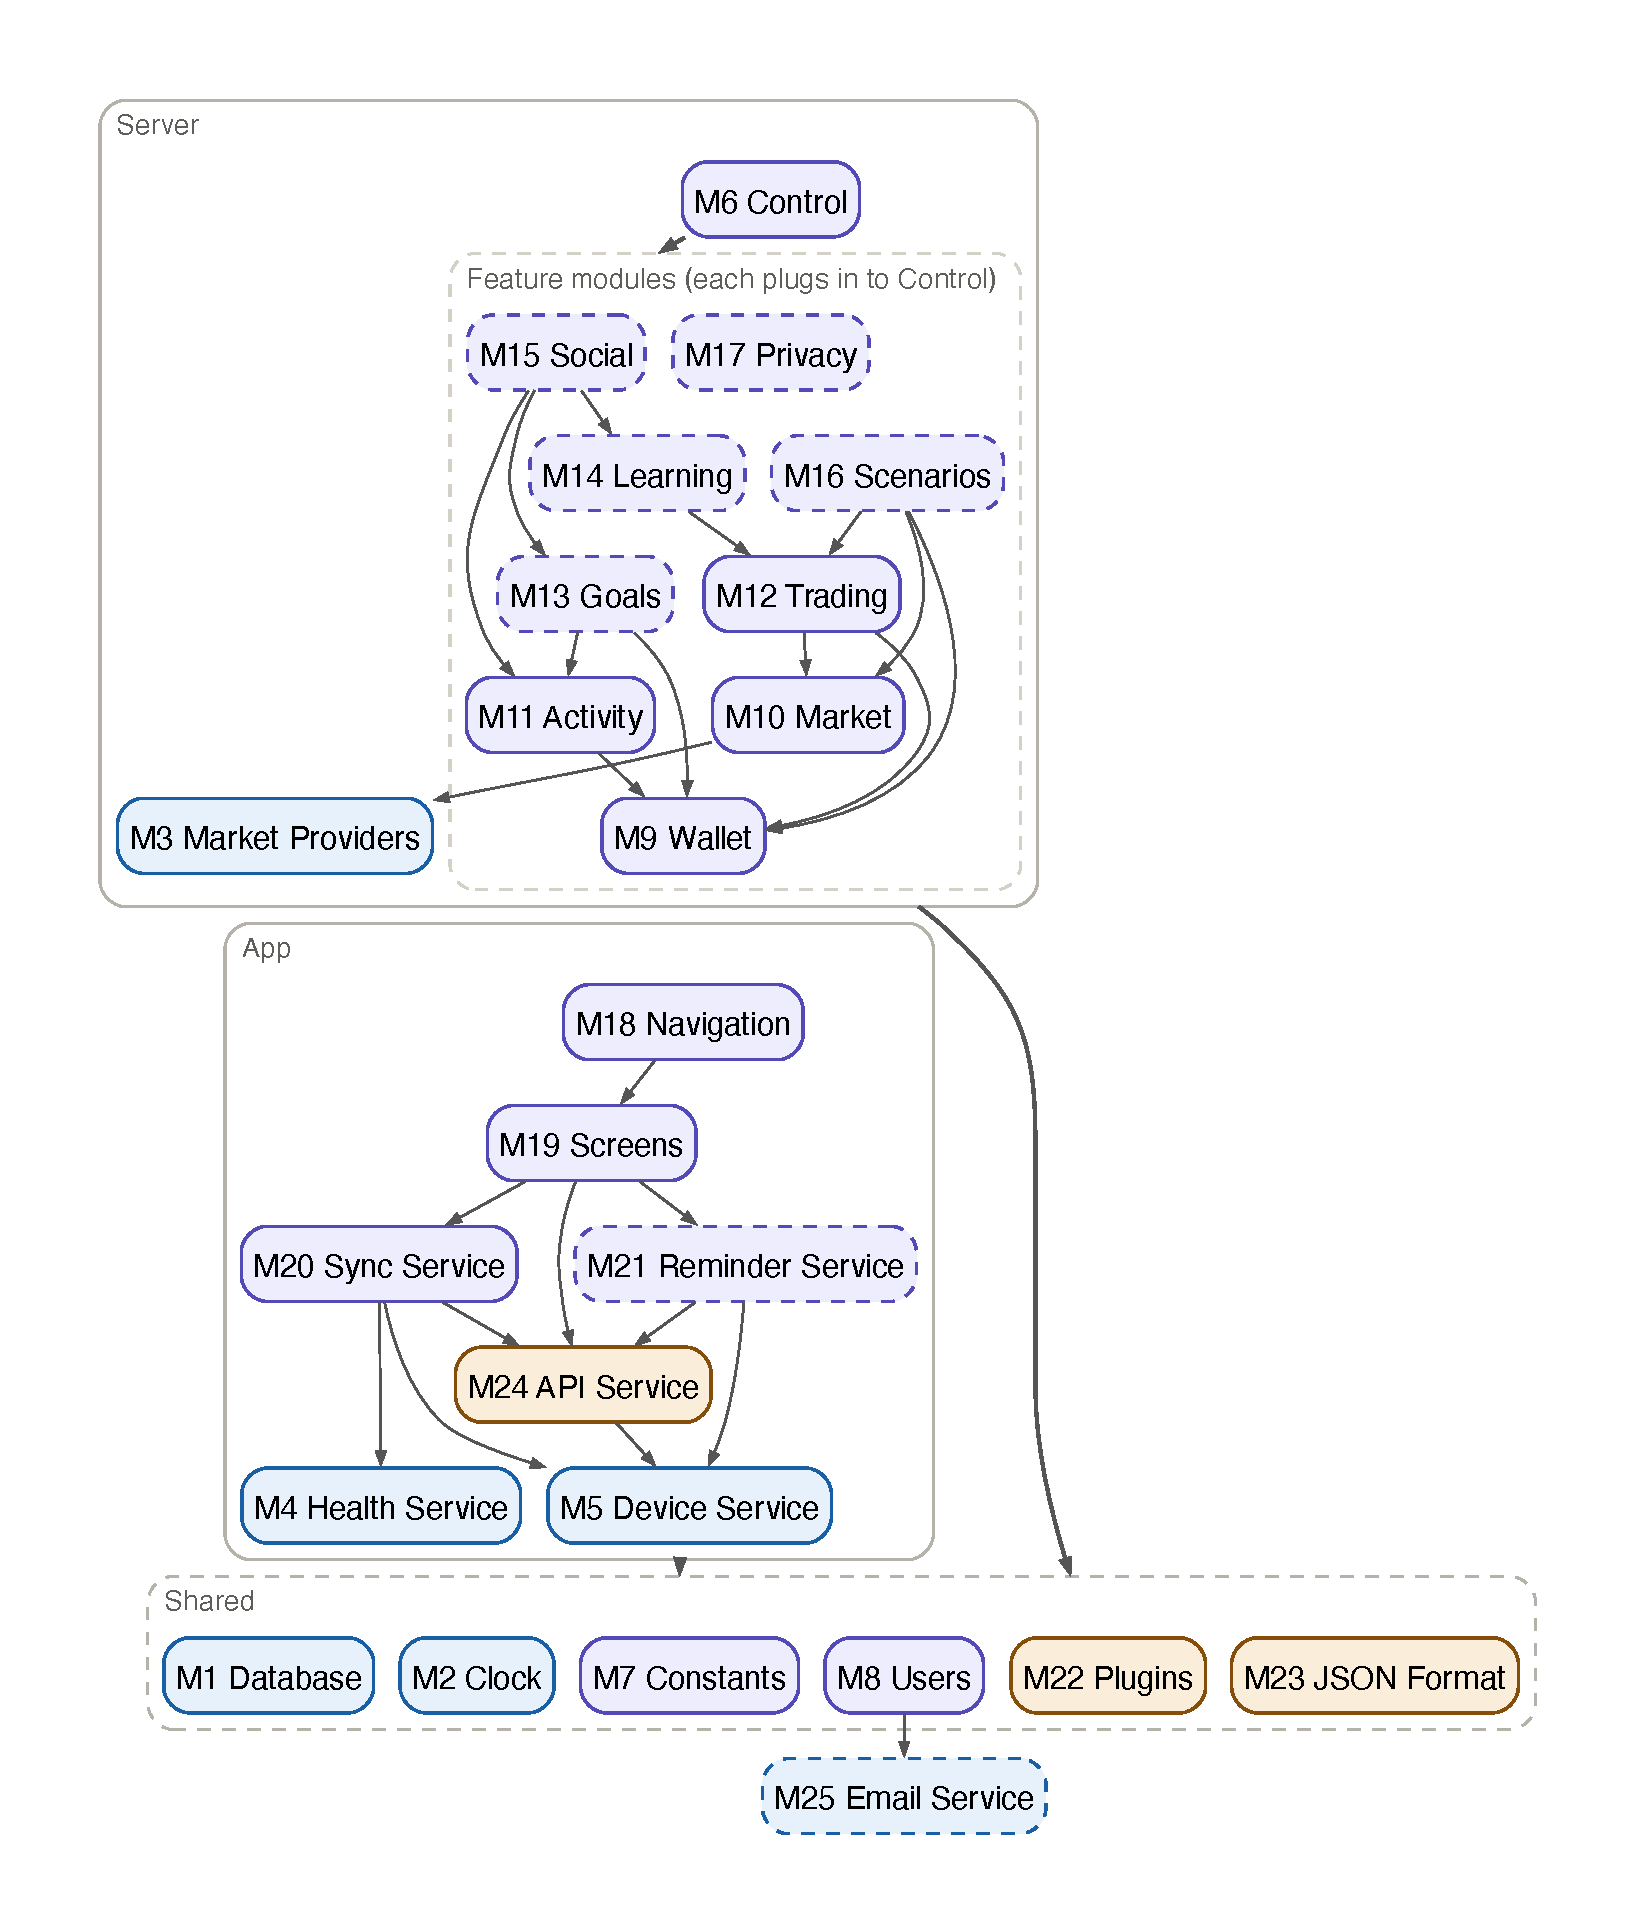
\includegraphics[width=\textwidth,height=0.9\textheight,keepaspectratio]{figures/uses-hierarchy.pdf}
\caption{Use hierarchy among modules. Blue: hardware-hiding. Purple:
behaviour-hiding. Orange: software decision. A dashed outline marks a module
built after the proof of concept.}
\label{FigUH}
\end{figure}

\begin{table}[H]
\centering
\begin{tabular}{p{0.35\textwidth} p{0.55\textwidth}}
\toprule
\textbf{Module} & \textbf{Uses}\\
\midrule
\mref{mDB} Database & None\\
\mref{mClock} Clock & None\\
\mref{mProviders} Market Providers & \mref{mClock}\\
\mref{mHealth} Health Service & None\\
\mref{mDevice} Device Service & None\\
\mref{mControl} Control & \mref{mDB}, \mref{mUsers}, \mref{mWallet}, \mref{mMarket}, \mref{mActivity}, \mref{mTrading}, \mref{mGoals}, \mref{mLearning}, \mref{mSocial}, \mref{mScenarios}, \mref{mPrivacy}, \mref{mPlugins}, \mref{mJSON}\\
\mref{mConstants} Constants & None\\
\mref{mUsers} Users & \mref{mDB}, \mref{mClock}, \mref{mConstants}, \mref{mPlugins}, \mref{mJSON}, \mref{mEmail}\\
\mref{mWallet} Wallet & \mref{mDB}, \mref{mUsers}, \mref{mPlugins}, \mref{mJSON}\\
\mref{mMarket} Market & \mref{mDB}, \mref{mClock}, \mref{mProviders}, \mref{mConstants}, \mref{mPlugins}, \mref{mJSON}\\
\mref{mActivity} Activity & \mref{mDB}, \mref{mClock}, \mref{mConstants}, \mref{mUsers}, \mref{mWallet}, \mref{mPlugins}, \mref{mJSON}\\
\mref{mTrading} Trading & \mref{mDB}, \mref{mClock}, \mref{mUsers}, \mref{mWallet}, \mref{mMarket}, \mref{mPlugins}, \mref{mJSON}\\
\mref{mGoals} Goals & \mref{mDB}, \mref{mClock}, \mref{mConstants}, \mref{mUsers}, \mref{mWallet}, \mref{mActivity}, \mref{mPlugins}, \mref{mJSON}\\
\mref{mLearning} Learning & \mref{mDB}, \mref{mConstants}, \mref{mUsers}, \mref{mTrading}, \mref{mPlugins}, \mref{mJSON}\\
\mref{mSocial} Social & \mref{mDB}, \mref{mClock}, \mref{mUsers}, \mref{mActivity}, \mref{mGoals}, \mref{mLearning}, \mref{mPlugins}, \mref{mJSON}\\
\mref{mScenarios} Scenarios & \mref{mDB}, \mref{mConstants}, \mref{mUsers}, \mref{mWallet}, \mref{mMarket}, \mref{mTrading}, \mref{mPlugins}, \mref{mJSON}\\
\mref{mPrivacy} Privacy & \mref{mDB}, \mref{mUsers}, \mref{mPlugins}, \mref{mJSON}\\
\mref{mNavigation} Navigation & \mref{mScreens}\\
\mref{mScreens} Screens & \mref{mConstants}, \mref{mSync}, \mref{mReminders}, \mref{mAPI}\\
\mref{mSync} Sync Service & \mref{mHealth}, \mref{mDevice}, \mref{mConstants}, \mref{mAPI}\\
\mref{mReminders} Reminder Service & \mref{mDevice}, \mref{mConstants}, \mref{mAPI}\\
\mref{mPlugins} Plugins & None\\
\mref{mJSON} JSON Format & None\\
\mref{mAPI} API Service & \mref{mDevice}\\
\mref{mEmail} Email Service & None\\
\bottomrule
\end{tabular}
\caption{Modules each module uses}
\label{TblUses}
\end{table}

%\section*{References}

\section{User Interfaces}

\wss{Design of user interface for software and hardware.  Attach an appendix if
needed. Drawings, Sketches, Figma}

\section{Design of Communication Protocols}

\wss{If there is communication between hardware and software, it may be necessary 
to explain the design of the communication protocol.  This section should be filled 
in with NA if it is not appropriate for a given project.}

\section{Database Design}

\wss{If a database is a significant component of the project, the database
design should be summarized here.  This section should be filled in with NA if
it is not appropriate for a given project.}

\section{Timeline}

\wss{Schedule of tasks and who is responsible}

\wss{You can point to GitHub if this information is included there}

\section{Generative AI Use Disclosure}

\wss{ChatGPT (version 5) was used to brainstorm ideas for the template for this disclose section.}

\subsection{AI Tools Used}

\wss{Give the name of the AI tool(s) used and the version.}

\subsection{How and Where Used}

\wss{Explain what the tool(s) were used for.  Examples include: brainstorming,
explaining a technical concept, reviewing the document, generating or modifying
text, generating or modifying diagrams, identifying errors or omissions or
inconsistencies.}

\wss{For each of the uses, identify which parts of the document were affected.}

\wss{You do not need to report every interaction, but you should disclose the 
uses that materially contributed to your work}

\subsection{Verification of AI-Generated Content}

\wss{\begin{itemize}
    \item Describe how the team checked AI-generated or AI-assisted material
    before including it in the document.
    \item In particular, verify factual claims, technical assertions,
    requirements, calculations, references, and other information for which an
    AI system may produce incorrect or fabricated results.
    \item \textbf{The team is responsible for the accuracy, completeness,
consistency, and appropriateness of the submitted document, regardless of
whether material was generated by a human or an AI system.}
\end{itemize}}

\end{document}